\chapter{Antecedentes}
En este capítulo se describirán los aspectos generales de los principales componentes del estudio. Primero se describirán diferentes algoritmos básicos usados para clasificación de series temporales. Tras esto se explicarán qué son las LSTM, su funcionamiento y estructura. Por último, se describirá el problema de desbalanceo de clases y diferentes enfoques para solucionarlo.\newline

\section{Clasificación de series temporales. Algoritmos Básicos}
\newpage
\section{LSTM}
Las LSTM ( Long Short-Term Memory ) son un tipo de red neuronal recurrente; este tipo de red es capaz de procesar de procesar secuencias de datos, como por ejemplo vídeos o frases. Este tipo de red neuronal se inventaron para ser usadas en problemas donde la información que se procesa es dependiente de información anteriormente procesada, y esta relación debe ser recordada hasta que deje de ser útil. Actualmente las redes con LSTM se utilizan en diversas tareas, como por ejemplo reconocimiento del habla, traducción, etc.\newline

Una unidad de LSTM o una neurona de LSTM tiene la siguiente estructura:
\begin{itemize}
	\item Puerta de entrada.
	\item Puerta de salida.
	\item Puerta de olvido.
	\item Célula.
\end{itemize}
\vspace{0.09in}
La célula es la encargada de almacenar información; el valor de la célula depende de los valores de las puertas de entrada, salida y olvido. Además, los valores de dichas puertas van cambiando en cada instante de tiempo. En la siguiente imagen se puede ver una representación de las estructura de una LSTM.\newline

\begin{figure}[h]
	\centering
	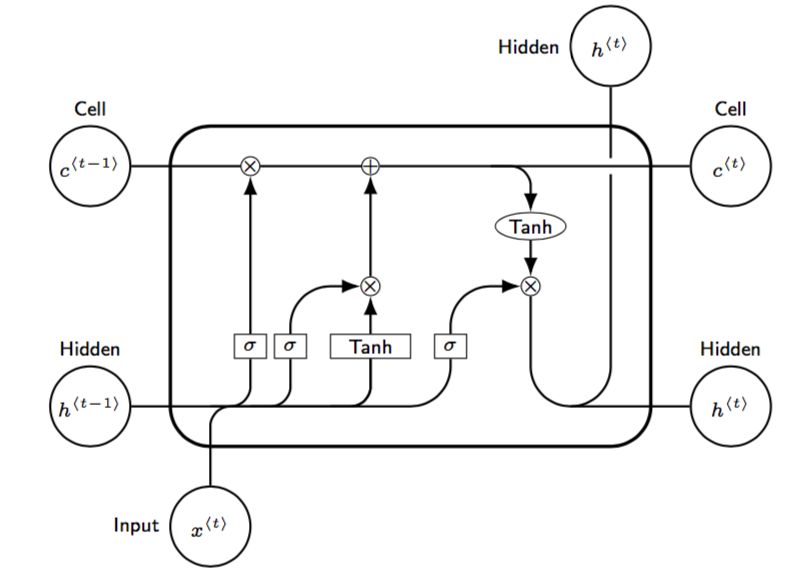
\includegraphics[width=120mm]{imagenes/lstm-struct.png}
	\label{fig:1}
	\caption{Estructura de una LSTM.}
\end{figure}
\vspace{0.09in}
La puerta de olvido tiene como función olvidar información anterior dependiendo de la información actual, dicha función podría expresarse de la siguiente forma.

$$ f^{(t)} = \sigma( W_f[h^{(t-1)}, x(t)] + b_f) $$

Donde:
\begin{itemize}
	\item $x^{(t)}$: entrada de la puerta en el momento $t$.
	\item $h^{(t-1)} $: valor de la salida de la célula en el instante anterior.
	\item $W_f $: matriz de pesos de la puerta de olvido.
	\item $b_f $: sesgo de la puerta de olvido.
	\item $\sigma$: función de activación (valores entre 0 y 1) de la puerta de olvido.
\end{itemize}
\vspace{0.09in}
La puerta de entrada tiene como función aprender los parámetros de entrada para su composición con el estado de la LSTM. PAra ello se debe calcular el estado de la LSTM y seleccionar la información que se utilizará para actualizar el estado. Esto se puede expresar mediante las siguientes funciones:\newline
$$ i^{(t)} = \sigma(W_i[h^{(t-1)}, x^{(t)}] + b_i) $$
$$ s'^{(t)} = \tanh(W_s[h^(t-1), x^{(t)}] + b_s) $$

Donde:
\begin{itemize}
	\item $s'^{(t)}$:estado local de la LSTM, sin tener en cuenta el estado anterior.
	\item $W_i$: matriz de pesos de la puerta de entrada.
	\item $W_s$: matriz de pesos del estado de la LSTM.
	\item $b_i $: sesgo de la puerta de entrada.
	\item $b_s$: sesgo del estado.
\end{itemize}
\verticalspace
Tras esto, se calcula el nuevo estado de la LSTM de la siguiente forma:\newline
$$ s^{(t)} = f^{(t)}s^{(t-1)} + i^{(t)} s'^{(t)} $$
De esta forma, el estado se forma con una parte del estado anterior, la que no se olvida; y con la composición de la entrada con el estado local ( $s'^{(t)}$ ).
\verticalspace

La puerta de salida es la encargada de aprender los parámetros de salida, esto puede expresarse mediante la siguiente función:\newline
$$ o^{(t)} = \sigma(W_o[h^{(t-1)}, x^{(t)}] + b_o) $$
Por último, la salida se calcula como:\newline
$$h^{(t)} = o^{(t)}\tanh(s^{(t)}) $$

La función para calcular la salida puede ser otra, como ReLu; las funciones de activación de las puertas también pueden ser otras.\newline

Como puede verse, las LSTM son capaces de guardar información relevante durante un largo periodo de tiempo y eliminar la información poco importante; por ello, son muy utilizadas en problemas con series temporales, ya que la información en un momento t es dependiente de la información que había en instantes anteriores y las LSTMs son capaces de detectar dicha dependencia y aprenderla.\newline

Las LSTM son un tipo de red recurrente, por lo que se pueden construir arquitecturas basadas en una LSTM que procesa la secuencia de izquierda a derecha y otra de derecha a izquierda; a estas estructuras se les llama LSTM bidireccionales, en la siguiente imagen se muestra un ejemplo de esta estructura.\newline
\newpage

\begin{figure}[h]
	\centering
	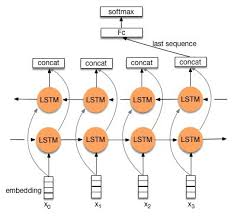
\includegraphics[width=85mm]{imagenes/bidi-lstm.jpg}
	\label{fig:2}
	\caption{Ejemplo de estructura de LSTM bidireccional.}
\end{figure}
\verticalspace
Gracias a este tipo de estructuras pueden resolverse problemas donde la importancia/sentido de un dato no depende de datos anteriores sino por información posterior; por ejemplo, el significado de una palabra puede ser diferente dependiendo de las palabras siguientes que haya en una secuencia y no en las anteriores.
\newpage
\section{Clasificación con clases no balanceadas}
El problema de desbalanceo de clases es un tipo de problema que aparece en problemas de clasificación. el desbalanceo de clases ocurre cuando el número de elementos de una clase es mucho mayor que el número de elementos de la otra clase; a esta clase se le llama clase minoritaria. En la siguiente imagen se puede ver un ejemplo en 2D de un problema de desbalanceo de clases.\newline

\begin{figure}[h]
	\centering
	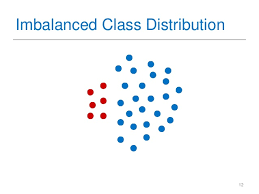
\includegraphics[width=85mm]{imagenes/imbalance_class.png}
	\label{fig:3}
	
\end{figure}
\verticalspace

El principal problema que tiene el desbalanceo de clases es que afecta a la capacidad de aprendizaje de la mayoría de los modelos de minería de datos actuales, exceptuando algunos como los árboles de decisión, aunque también trabajan mejor si no hay desbalanceo. Además, si el desbalanceo es muy grande es posible que los modelos no aprendan directamente la clase minoritaria.\newline

Otro problema es que afecta a las medidas utilizadas normalmente en problemas de clasificación como es el Accuracy; esta medida representa el número de elementos bien clasificados sobre el total de elementos; si por ejemplo la clase minoritaria representa el 0.1\% de los datos y un clasificador predijera todos los datos como elementos de la clase mayoritaria, su Accuracy sería del 99.9\%; por ello, se debe utilizar otras medidas. Las medidas usuales son Precision, Recall, AUC, G-Mean, F1-Score, etc; todas estas medidas tienen en cuenta la clase minoritaria de forma que si ocurre lo anterior su valor sea bajo.\newline

Como solución al problema del desbalanceo existen dos propuestas, una basada en modificación de algoritmos y otra basada en modificación del conjunto de datos.
\subsection{Técnicas basadas en modificación del algoritmo}
Este enfoque se centra en modificar clasificadores ya existentes para aliviar el sesgo hacia la clase mayoritaria en vez de alterar el conjunto de datos. Esto requiere un buen conocimiento interno del modelo que se quiere modificar y saber las razones por las cuales falla al identificar la clase minoritaria.\newline

Modificar un modelo reduce su flexibilidad y por lo tanto lo hace válido para un número menor de problemas, pero a cambio ofrece una mayor especialización para el tipo de problema que se modifica.\newline

Algunos ejemplos de modelos modificados son árboles de decisión que utilizan la distancia de Hellinger para la separación de nodos, utilizar un método diferente de cálculo de pertenencia de clases para KNN, por ejemplo con pesos en vez de distancias, uso de kernels específicos con SVM, etc.\newline

\begin{figure}[h]
	\centering
	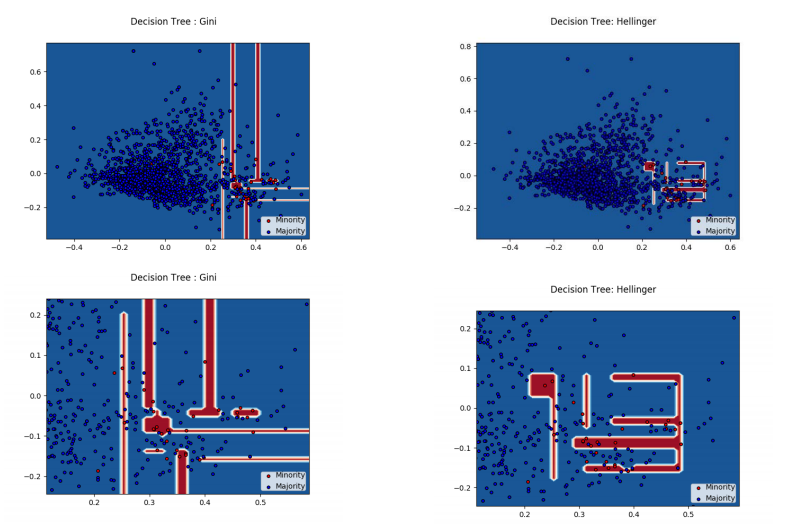
\includegraphics[width=100mm]{imagenes/hellinger-example.png}
	\label{fig:4}
	\caption{Ejemplo comportamiento algoritmo.}
\end{figure}
\verticalspace

Otra posible solución es modificar el peso asociado a clasificar mal un elemento, dando un peso mayor a clasificar mal un elemento de la clase minoritaria que de la mayoritaria, de forma que cuando se entrena el modelo intenta minimizarse el coste. El peso asociado a cada fallo se almacena en la matriz de costes, dicha matriz puede ser calculada con diferentes heurísticas o aportada por un experto en el problema que se plantee. El la siguiente imagen se muestra un ejemplo del uso de la matriz de costes para un clasificador simple.\newline

\begin{figure}[h]
	\centering
	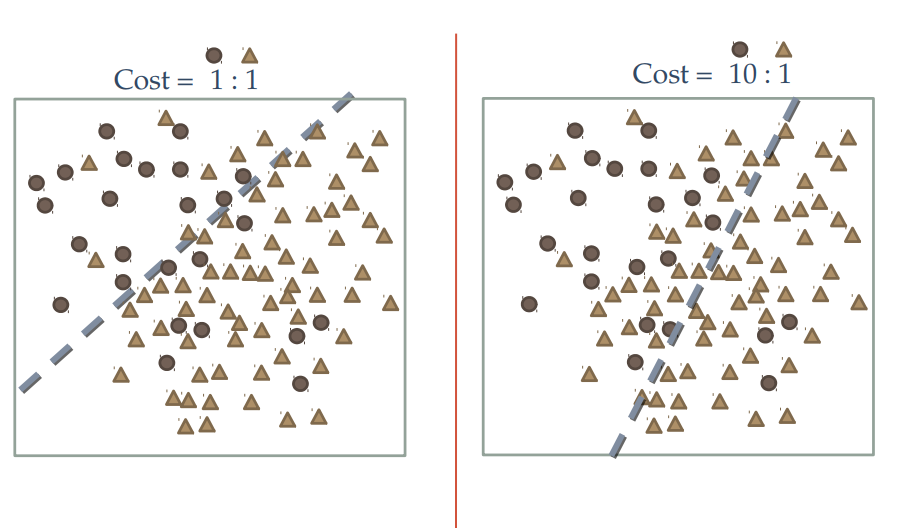
\includegraphics[width=90mm]{imagenes/cost-sentitive.png}
	\label{fig:5}
\end{figure}
\verticalspace

Existen dos formas de usar la matriz de costes, la primera es integrar el uso de la matriz dentro del algoritmo, lo que significa que hay modificarlo para que use dicha matriz; la segunda forma es preprocesando los datos de entrada asignándole un peso o asignando a cada elemento la clase que se cree que tendrá menor coste (para ello se hace uso del Teorema de Bayes).
\subsection{Técnicas basadas en la modificación del conjunto de datos}
La idea de este tipo de técnica es manipular la distribución de los datos con los que entrena el clasificador, para ello se añaden o suprimen elementos del conjunto de datos. Cuando se añaden elementos, se llama “oversampling” y cuando eliminan “undersampling”; dependiendo del problem se puede usar una de estas técnicas o ambas.\newline
\newpage
\begin{figure}[h]
	\centering
	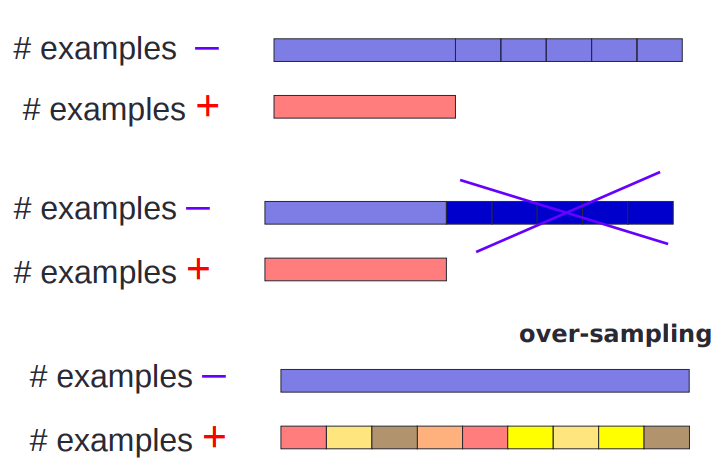
\includegraphics[width=110mm]{imagenes/oversampling_undersampling.png}
	\label{fig:6}
\end{figure}
\verticalspace

Un ejemplo clásico de algoritmo de undersampling es Tomek Links; este algoritmo elimina elementos de la clase mayoritaria que sean fronterizos con elementos de la clase minoritaria; para ello calcula las parejas de elementos de clases diferentes que estén a la distancia mínima entre ellos, es decir, que no haya ningún otro elemento dentro del conjunto de datos que su distancia hacia ese elemento sea menor; y elimina aquellos que sean de la clase mayoritaria. En la siguiente imagen se muestra un ejemplo del uso de este algoritmo.\newline


\begin{figure}[h]
	\centering
	
\includegraphics[width=120mm]{imagenes/tomek-example.png}
	\label{fig:7}
	\caption{Ejemplo funcionamiento algoritmo Tomek-Links.}
\end{figure}
\verticalspace

Otros métodos de undersampling son OSS, CNN y combinaciones de ellos. El problema del undersampling es que al eliminar elementos de la clase mayoritaria hace que cierta información se pierda, y dicha información puede ser importante al evaluar.\newline

Un algoritmo clásico de oversampling es SMOTE, este algoritmo crea nuevas instancias usando una combinación de K instancias de la clase minoritaria que sean vecinas. En la siguiente imagen se muestra un ejemplo del funcionamiento del SMOTE.\newline

\begin{figure}[h]
	\centering
	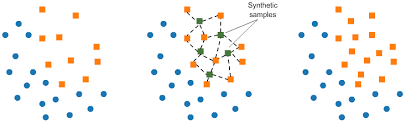
\includegraphics[width=120mm]{imagenes/smote-example.png}
	\label{fig:8}
	\caption{Ejemplo funcionamiento algoritmo SMOTE.}
\end{figure}
\verticalspace

Otros algoritmos de oversampling son modificaciones de SMOTE, como por ejemplo Borderline-SMOTE (centrado en la generación de instancias en la frontera), ADASYN, etc.\newline

El problema del oversampling es que pueden generalizar demasiado la clase minoritaria y provocar ruido en el conjunto de datos.

\subsection{Otros enfoques}
Una última opción para paliar el desbalanceo sin implicar modificaciones de los algoritmos o del subconjunto de datos, esta es el uso de modelos ensemble; los modelos ensemble son aquellos que están formados por varios modelos más simples, para ello, los modelos simples se entrenan con un subconjunto de los datos, de forma que en esos subconjuntos el desbalanceo no tiene porque ser tan grande. Para elegir una clase, los modelos ensemble pueden combinar los resultados de los modelos simples ( para problemas de regresión ) o mediante voto. Un ejemplo de modelo ensemble es RandomForest.